\begin{frame}
\frametitle{Simplifications / Terme de rigidité / Gradient}
\vfill
\begin{columns}%[c]
\column{.5\textwidth}
\begin{itemize}
\item Pour une fonction de base $\PsiRef{i}$ donnée, la valeur de son gradient
en un point d'intégration $\GLN{j}$ est non nulle uniquement si ce point est aligné dans une direction avec le point
$\GLN{i}$ associé à la fonction ;
\item<5-> Seule la composante correspondant à la direction d'alignement est non nulle ;
\end{itemize}
\column{.5\textwidth}
\begin{figure}
\centering
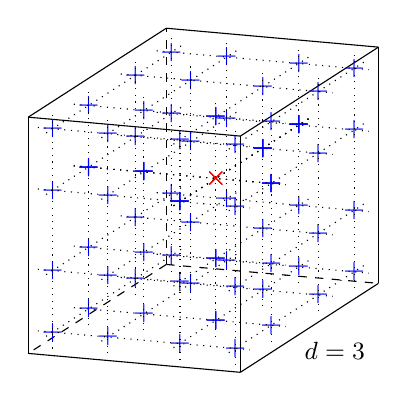
\begin{tikzpicture}[scale=3,rotate around x=270,rotate around z=258]
	% cube
	\draw [dashed] (0,0,0) -- (1,0,0);
	\draw [dashed] (0,0,0) -- (0,1,0);
	\draw [dashed] (0,0,0) -- (0,0,1);

	\draw [-] (1,1,0) -- (1,0,0);
	\draw [-] (0,1,1) -- (0,1,0);
	\draw [-] (1,0,1) -- (0,0,1);

	\draw [-] (1,1,0) -- (0,1,0);
	\draw [-] (0,1,1) -- (0,0,1);
	\draw [-] (1,0,1) -- (1,0,0);

	\draw [-] (1,1,0) -- (1,1,1);
	\draw [-] (0,1,1) -- (1,1,1);
	\draw [-] (1,0,1) -- (1,1,1);
	
	\draw (0.7,1.25) node {\small$d=3$};

\onslide<1>{
	% gauss legendre: 0.06943, 0.33, 0.67, 0.9306
	\def \rpg {0.67}
	\def \pgs {0.06943,0.33,0.9306}
	% points volumiques
	\foreach \x in \pgs {
	\foreach \y in \pgs {
	\foreach \z in \pgs {
		\draw (\x,\y,\z) node[blue] {$\bm{+}$};
	}}}
	\foreach \y in \pgs {
	\foreach \z in \pgs {
		\draw (\rpg,\y,\z) node[blue] {$\bm{+}$};
	}}
	\foreach \x in \pgs {
	\foreach \z in \pgs {
		\draw (\x,\rpg,\z) node[blue] {$\bm{+}$};
	}}
	\foreach \x in \pgs {
	\foreach \y in \pgs {
		\draw (\x,\y,\rpg) node[blue] {$\bm{+}$};
	}}
	% points volumiques alignés
	\foreach \x in \pgs {
		\draw (\x,\rpg,\rpg) node[blue] {$\bm{+}$};
		\draw (\rpg,\x,\rpg) node[blue] {$\bm{+}$};
		\draw (\rpg,\rpg,\x) node[blue] {$\bm{+}$};
	}
	% point volumique de référence
	\draw (\rpg,\rpg,\rpg) node[red] {$\bm{\times}$};

	\def \apgs {0.06943,0.33,0.67,0.9306}
	% points surface et lignes pointilées direction x
	\foreach \y in \apgs
	\foreach \z in \apgs {
		\draw [dotted] (0,\y,\z) -- (1,\y,\z);
%		\foreach \x in \c {
%			\draw (\x,\y,\z) node[green] {$\bm{\times}$};
%		}
	}
	% points surface et lignes pointilées direction y
	\foreach \x in \apgs
	\foreach \z in \apgs {
		\draw [dotted] (\x,0,\z) -- (\x,1,\z);
%		\foreach \y in \c {
%			\draw (\x,\y,\z) node[green] {$\bm{\times}$};
%		}
	}
	% points surface et lignes pointilées direction z
	\foreach \x in \apgs
	\foreach \y in \apgs {
		\draw [dotted] (\x,\y,0) -- (\x,\y,1);
%		\foreach \z in \c {
%			\draw (\x,\y,\z) node[green] {$\bm{\times}$};
%		}
	}
}
\onslide<2>{
	% gauss legendre: 0.06943, 0.33, 0.67, 0.9306
	\def \rpg {0.67}
	\def \pgs {0.06943,0.33,0.9306}
	% pointillés
	\draw [dotted] (0,\rpg,\rpg) -- (1,\rpg,\rpg);
	% points volumiques alignés
	\foreach \x in \pgs {
		\draw (\x,\rpg,\rpg) node[blue] {$\bm{+}$};
	}
	% point volumique de référence
	\draw (\rpg,\rpg,\rpg) node[red] {$\bm{\times}$};
}
\onslide<3>{
	% gauss legendre: 0.06943, 0.33, 0.67, 0.9306
	\def \rpg {0.67}
	\def \pgs {0.06943,0.33,0.9306}
	% pointillés
	\draw [dotted] (0,\rpg,\rpg) -- (1,\rpg,\rpg);
	\draw [dotted] (\rpg,0,\rpg) -- (\rpg,1,\rpg);
	% points volumiques alignés
	\foreach \x in \pgs {
		\draw (\x,\rpg,\rpg) node[blue] {$\bm{+}$};
		\draw (\rpg,\x,\rpg) node[blue] {$\bm{+}$};
	}
	% point volumique de référence
	\draw (\rpg,\rpg,\rpg) node[red] {$\bm{\times}$};
}
\onslide<4->{
	% gauss legendre: 0.06943, 0.33, 0.67, 0.9306
	\def \rpg {0.67}
	\def \pgs {0.06943,0.33,0.9306}
	% pointillés
	\draw [dotted] (0,\rpg,\rpg) -- (1,\rpg,\rpg);
	\draw [dotted] (\rpg,0,\rpg) -- (\rpg,1,\rpg);
	\draw [dotted] (\rpg,\rpg,0) -- (\rpg,\rpg,1);
	% points volumiques alignés
	\foreach \x in \pgs {
		\draw (\x,\rpg,\rpg) node[blue] {$\bm{+}$};
		\draw (\rpg,\x,\rpg) node[blue] {$\bm{+}$};
		\draw (\rpg,\rpg,\x) node[blue] {$\bm{+}$};
	}
	% point volumique de référence
	\draw (\rpg,\rpg,\rpg) node[red] {$\bm{\times}$};
}
\end{tikzpicture}
\end{figure}
\end{columns}
\vfill
\begin{itemize}
\item<6-> Complexité du terme de rigidité pour une fonction de base :\\
$(\Deg + 1)^3$ opérations vectorielles $\rightarrow$ $3 (\Deg + 1)$ opérations scalaires.
\end{itemize}
\vfill
\end{frame}

